% Options for packages loaded elsewhere
\PassOptionsToPackage{unicode}{hyperref}
\PassOptionsToPackage{hyphens}{url}
%
\documentclass[
]{article}
\title{Kahan scale and Economic Political value scale}
\author{}
\date{\vspace{-2.5em}}

\usepackage{amsmath,amssymb}
\usepackage{lmodern}
\usepackage{iftex}
\ifPDFTeX
  \usepackage[T1]{fontenc}
  \usepackage[utf8]{inputenc}
  \usepackage{textcomp} % provide euro and other symbols
\else % if luatex or xetex
  \usepackage{unicode-math}
  \defaultfontfeatures{Scale=MatchLowercase}
  \defaultfontfeatures[\rmfamily]{Ligatures=TeX,Scale=1}
\fi
% Use upquote if available, for straight quotes in verbatim environments
\IfFileExists{upquote.sty}{\usepackage{upquote}}{}
\IfFileExists{microtype.sty}{% use microtype if available
  \usepackage[]{microtype}
  \UseMicrotypeSet[protrusion]{basicmath} % disable protrusion for tt fonts
}{}
\makeatletter
\@ifundefined{KOMAClassName}{% if non-KOMA class
  \IfFileExists{parskip.sty}{%
    \usepackage{parskip}
  }{% else
    \setlength{\parindent}{0pt}
    \setlength{\parskip}{6pt plus 2pt minus 1pt}}
}{% if KOMA class
  \KOMAoptions{parskip=half}}
\makeatother
\usepackage{xcolor}
\IfFileExists{xurl.sty}{\usepackage{xurl}}{} % add URL line breaks if available
\IfFileExists{bookmark.sty}{\usepackage{bookmark}}{\usepackage{hyperref}}
\hypersetup{
  pdftitle={Kahan scale and Economic Political value scale},
  hidelinks,
  pdfcreator={LaTeX via pandoc}}
\urlstyle{same} % disable monospaced font for URLs
\usepackage[margin=1in]{geometry}
\usepackage{graphicx}
\makeatletter
\def\maxwidth{\ifdim\Gin@nat@width>\linewidth\linewidth\else\Gin@nat@width\fi}
\def\maxheight{\ifdim\Gin@nat@height>\textheight\textheight\else\Gin@nat@height\fi}
\makeatother
% Scale images if necessary, so that they will not overflow the page
% margins by default, and it is still possible to overwrite the defaults
% using explicit options in \includegraphics[width, height, ...]{}
\setkeys{Gin}{width=\maxwidth,height=\maxheight,keepaspectratio}
% Set default figure placement to htbp
\makeatletter
\def\fps@figure{htbp}
\makeatother
\setlength{\emergencystretch}{3em} % prevent overfull lines
\providecommand{\tightlist}{%
  \setlength{\itemsep}{0pt}\setlength{\parskip}{0pt}}
\setcounter{secnumdepth}{-\maxdimen} % remove section numbering
\ifLuaTeX
  \usepackage{selnolig}  % disable illegal ligatures
\fi

\begin{document}
\maketitle

{
\setcounter{tocdepth}{2}
\tableofcontents
}
\newpage

\hypertarget{exploratory-data-analysis}{%
\section{Exploratory Data analysis}\label{exploratory-data-analysis}}

\textbf{Distributions for DVs} I started by exploring the distributions
of perceived risk across various energy technologies. Below are boxplot
and violin plot for the same. We see that these are not normal
distributions.

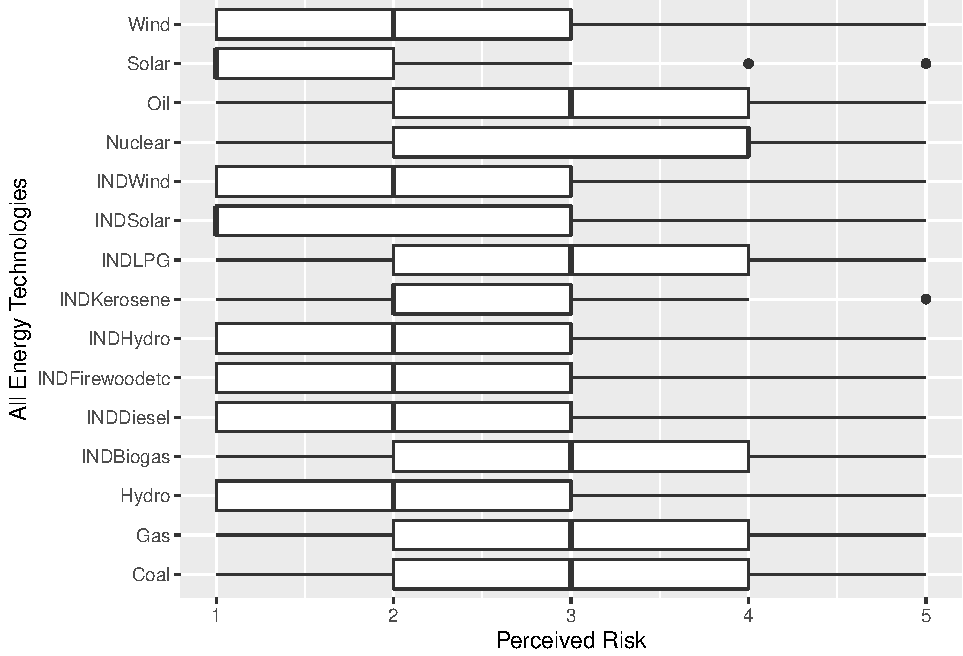
\includegraphics{Significant_results_files/figure-latex/unnamed-chunk-5-1.pdf}
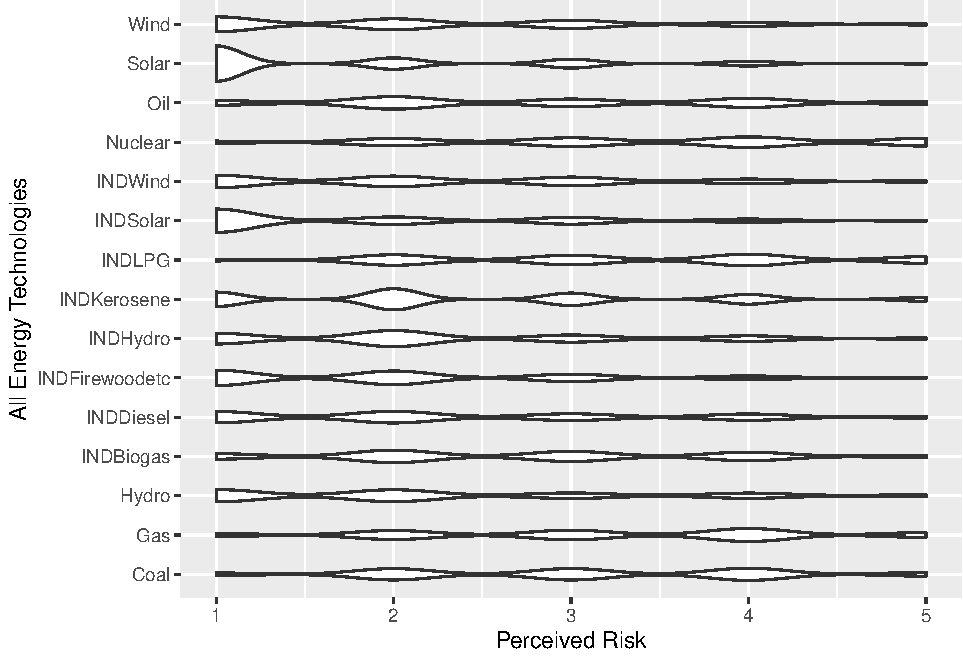
\includegraphics{Significant_results_files/figure-latex/unnamed-chunk-5-2.pdf}

\newpage

\hypertarget{how-much-is-the-awareness-of-energy-technologies-in-india-how-does-it-relate-to-state-specific-data}{%
\section{How much is the awareness of energy technologies in India ? How
does it relate to state specific data
?}\label{how-much-is-the-awareness-of-energy-technologies-in-india-how-does-it-relate-to-state-specific-data}}

To answer this I simply plotted the risk and benefit responses in a bar
graph. This will reveal the Rather not say/Do not know part of the
responses as well.

The percentages are rounded off to whole numbers.

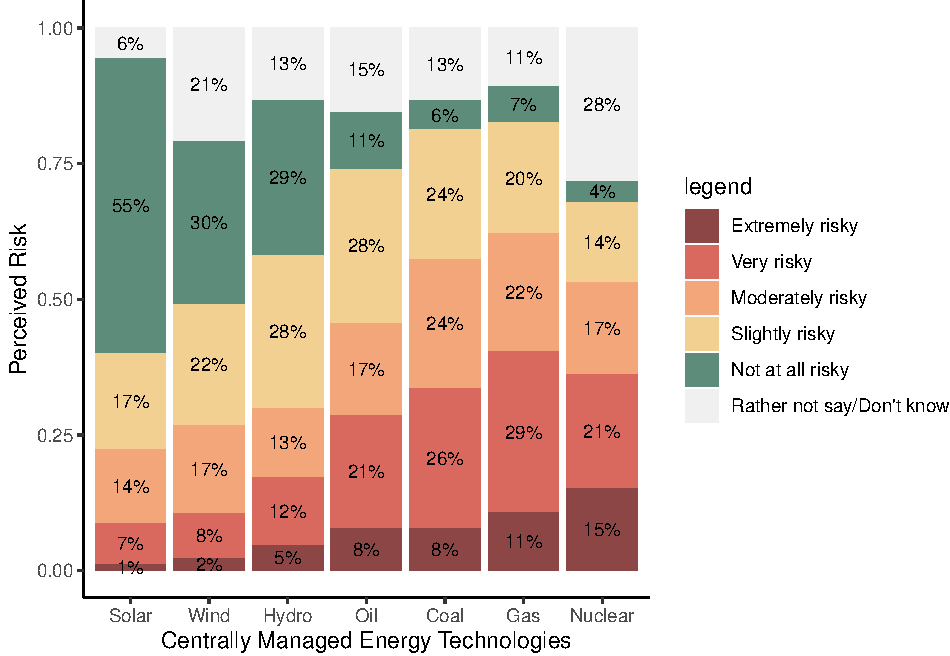
\includegraphics{Significant_results_files/figure-latex/unnamed-chunk-6-1.pdf}
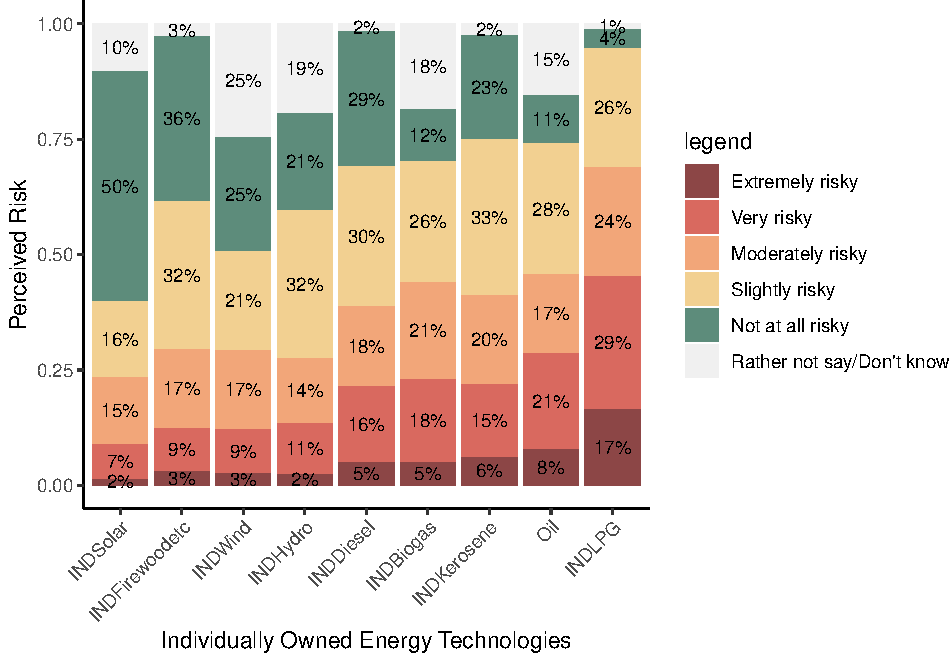
\includegraphics{Significant_results_files/figure-latex/unnamed-chunk-6-2.pdf}

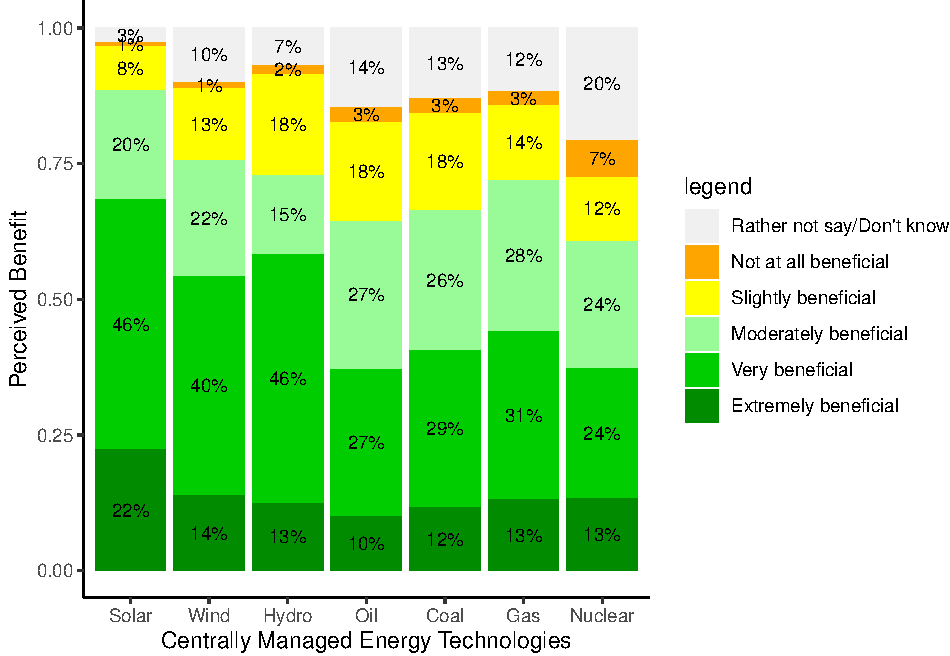
\includegraphics{Significant_results_files/figure-latex/unnamed-chunk-7-1.pdf}
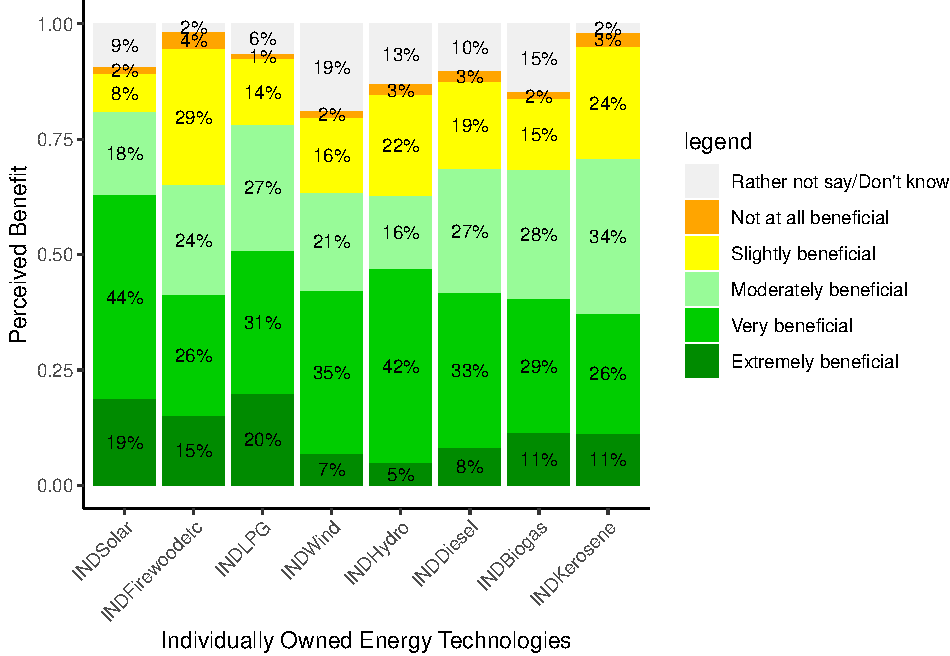
\includegraphics{Significant_results_files/figure-latex/unnamed-chunk-7-2.pdf}

\newpage

\hypertarget{state-specific-perceived-risk-and-perceived-benefit-from-centrally-managed-energy-technologies.}{%
\section{State Specific perceived risk and perceived benefit from
Centrally Managed energy
technologies.}\label{state-specific-perceived-risk-and-perceived-benefit-from-centrally-managed-energy-technologies.}}

The percentage of Rather not say/Do not know differs for each technology
from state to state. This graph explores that. The number of respondents
from each state are also reported below.

\begin{verbatim}
##   Maharashtra     Rajasthan    Tamil Nadu Uttar Pradesh   West Bengal 
##           653           677           320           125           386
\end{verbatim}

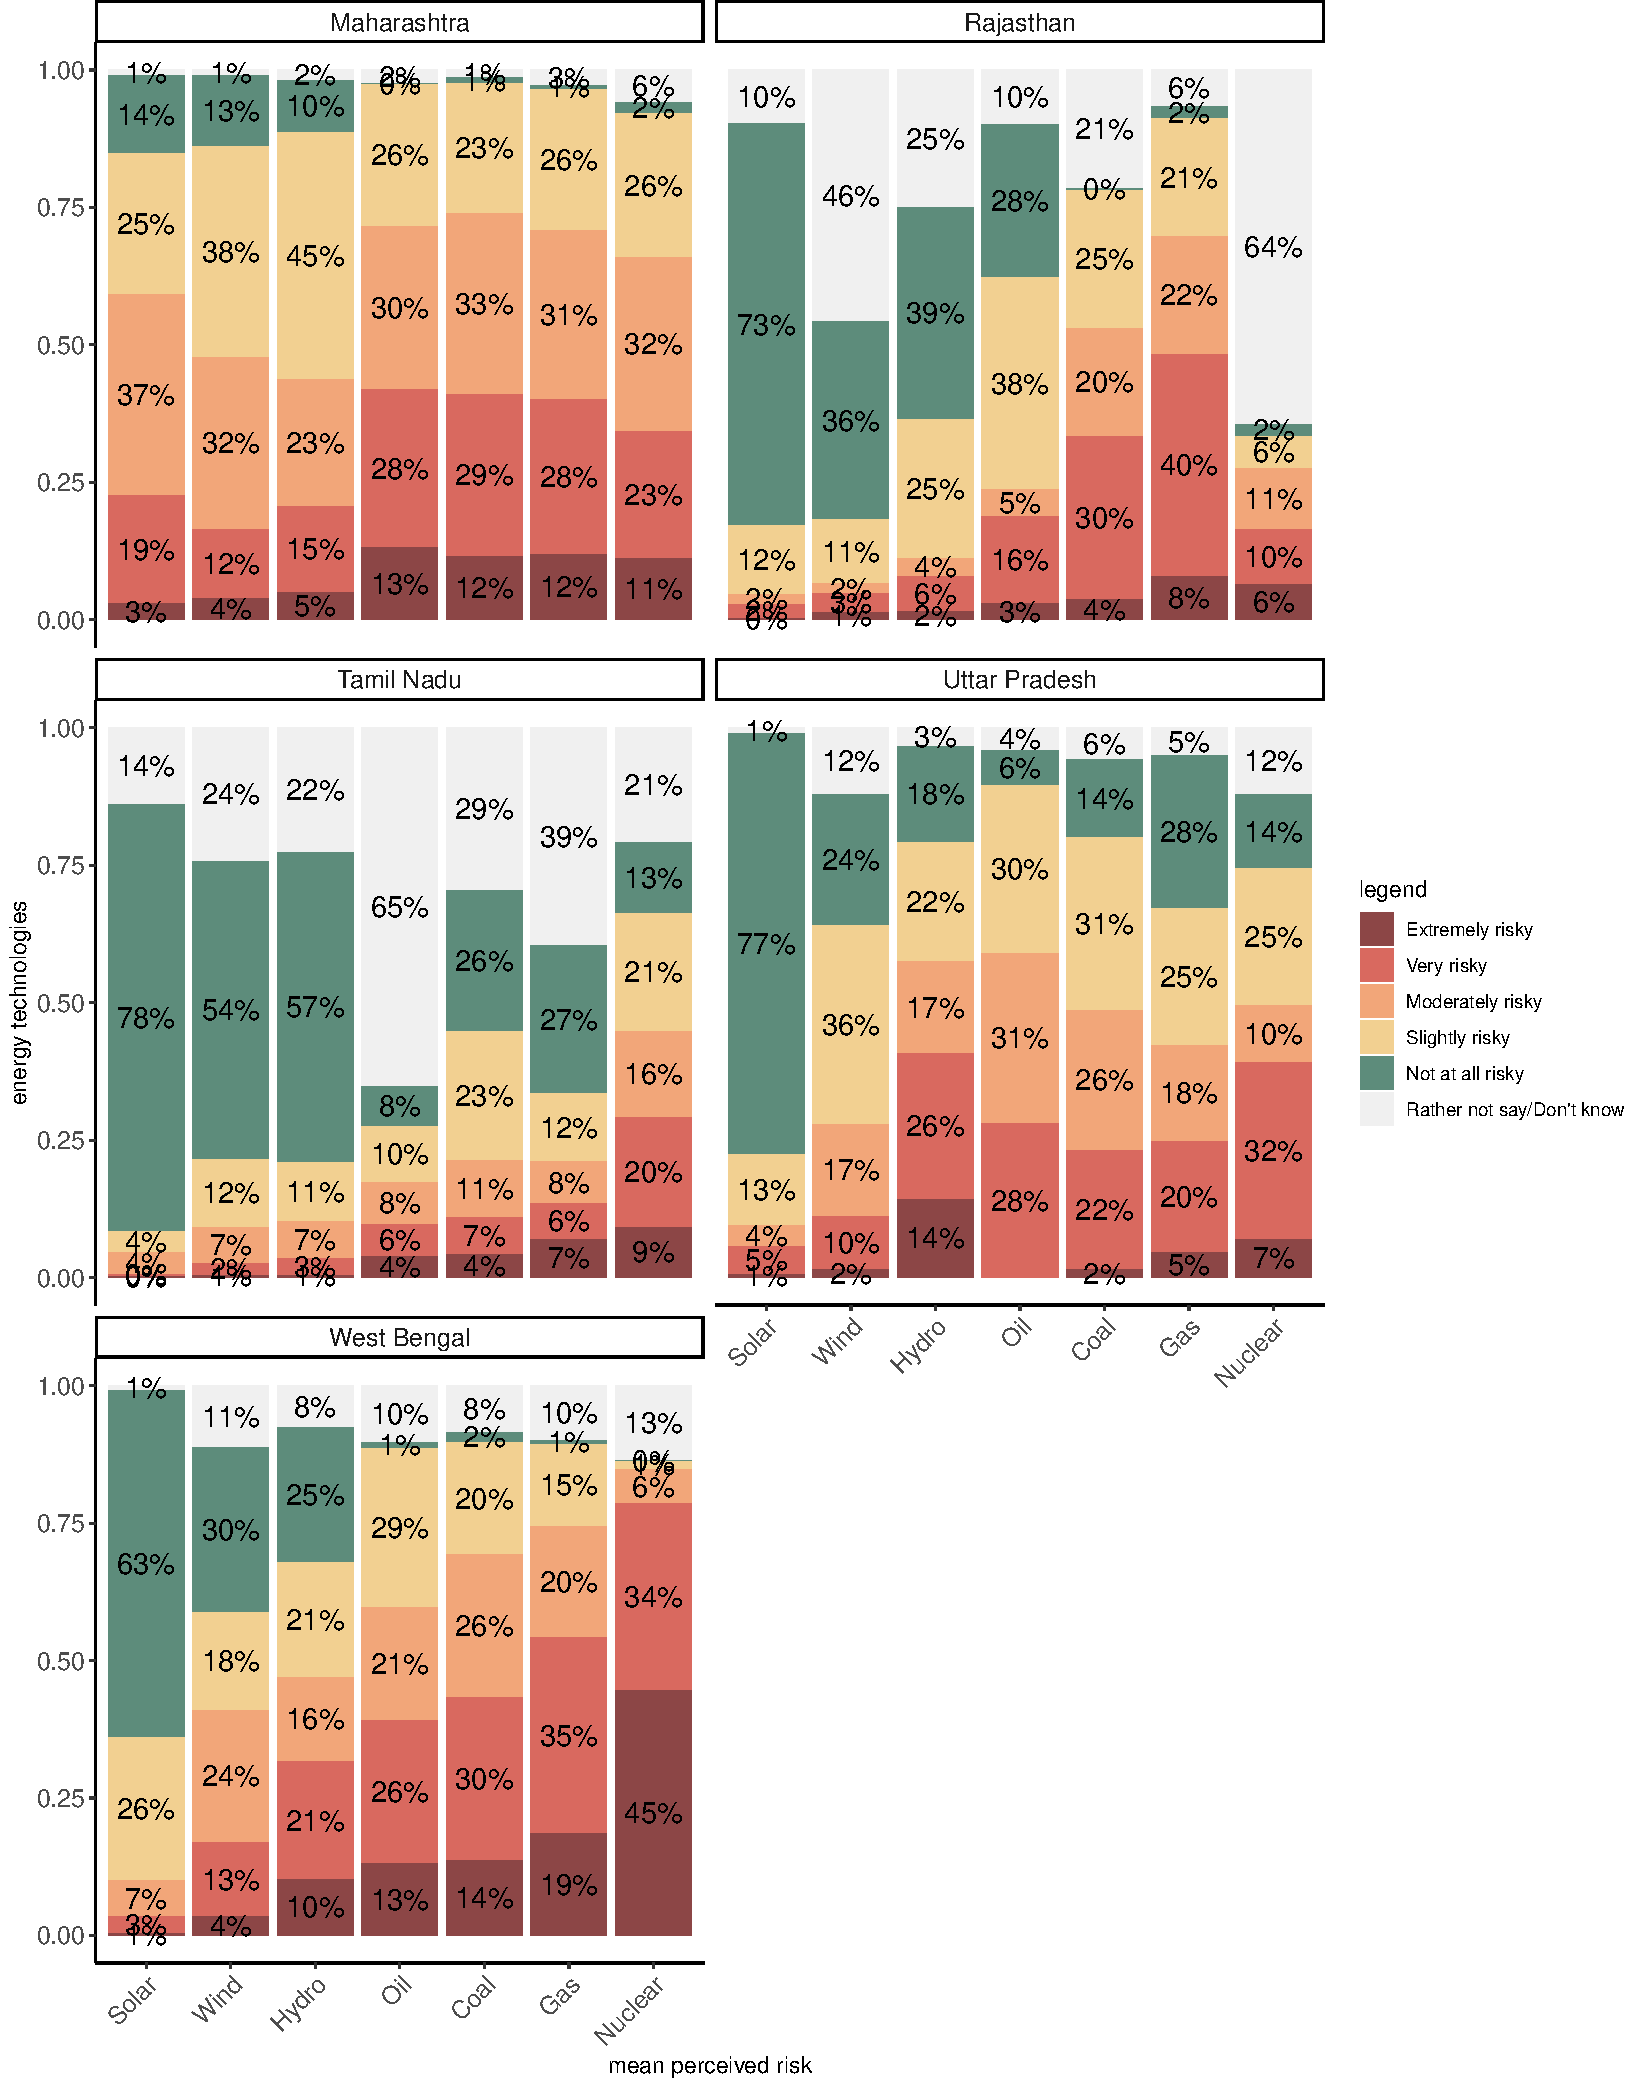
\includegraphics[width=0.7\linewidth,height=0.7\textheight]{Significant_results_files/figure-latex/unnamed-chunk-8-1}

\newpage

\begin{verbatim}
##   Maharashtra     Rajasthan    Tamil Nadu Uttar Pradesh   West Bengal 
##           653           677           320           125           386
\end{verbatim}

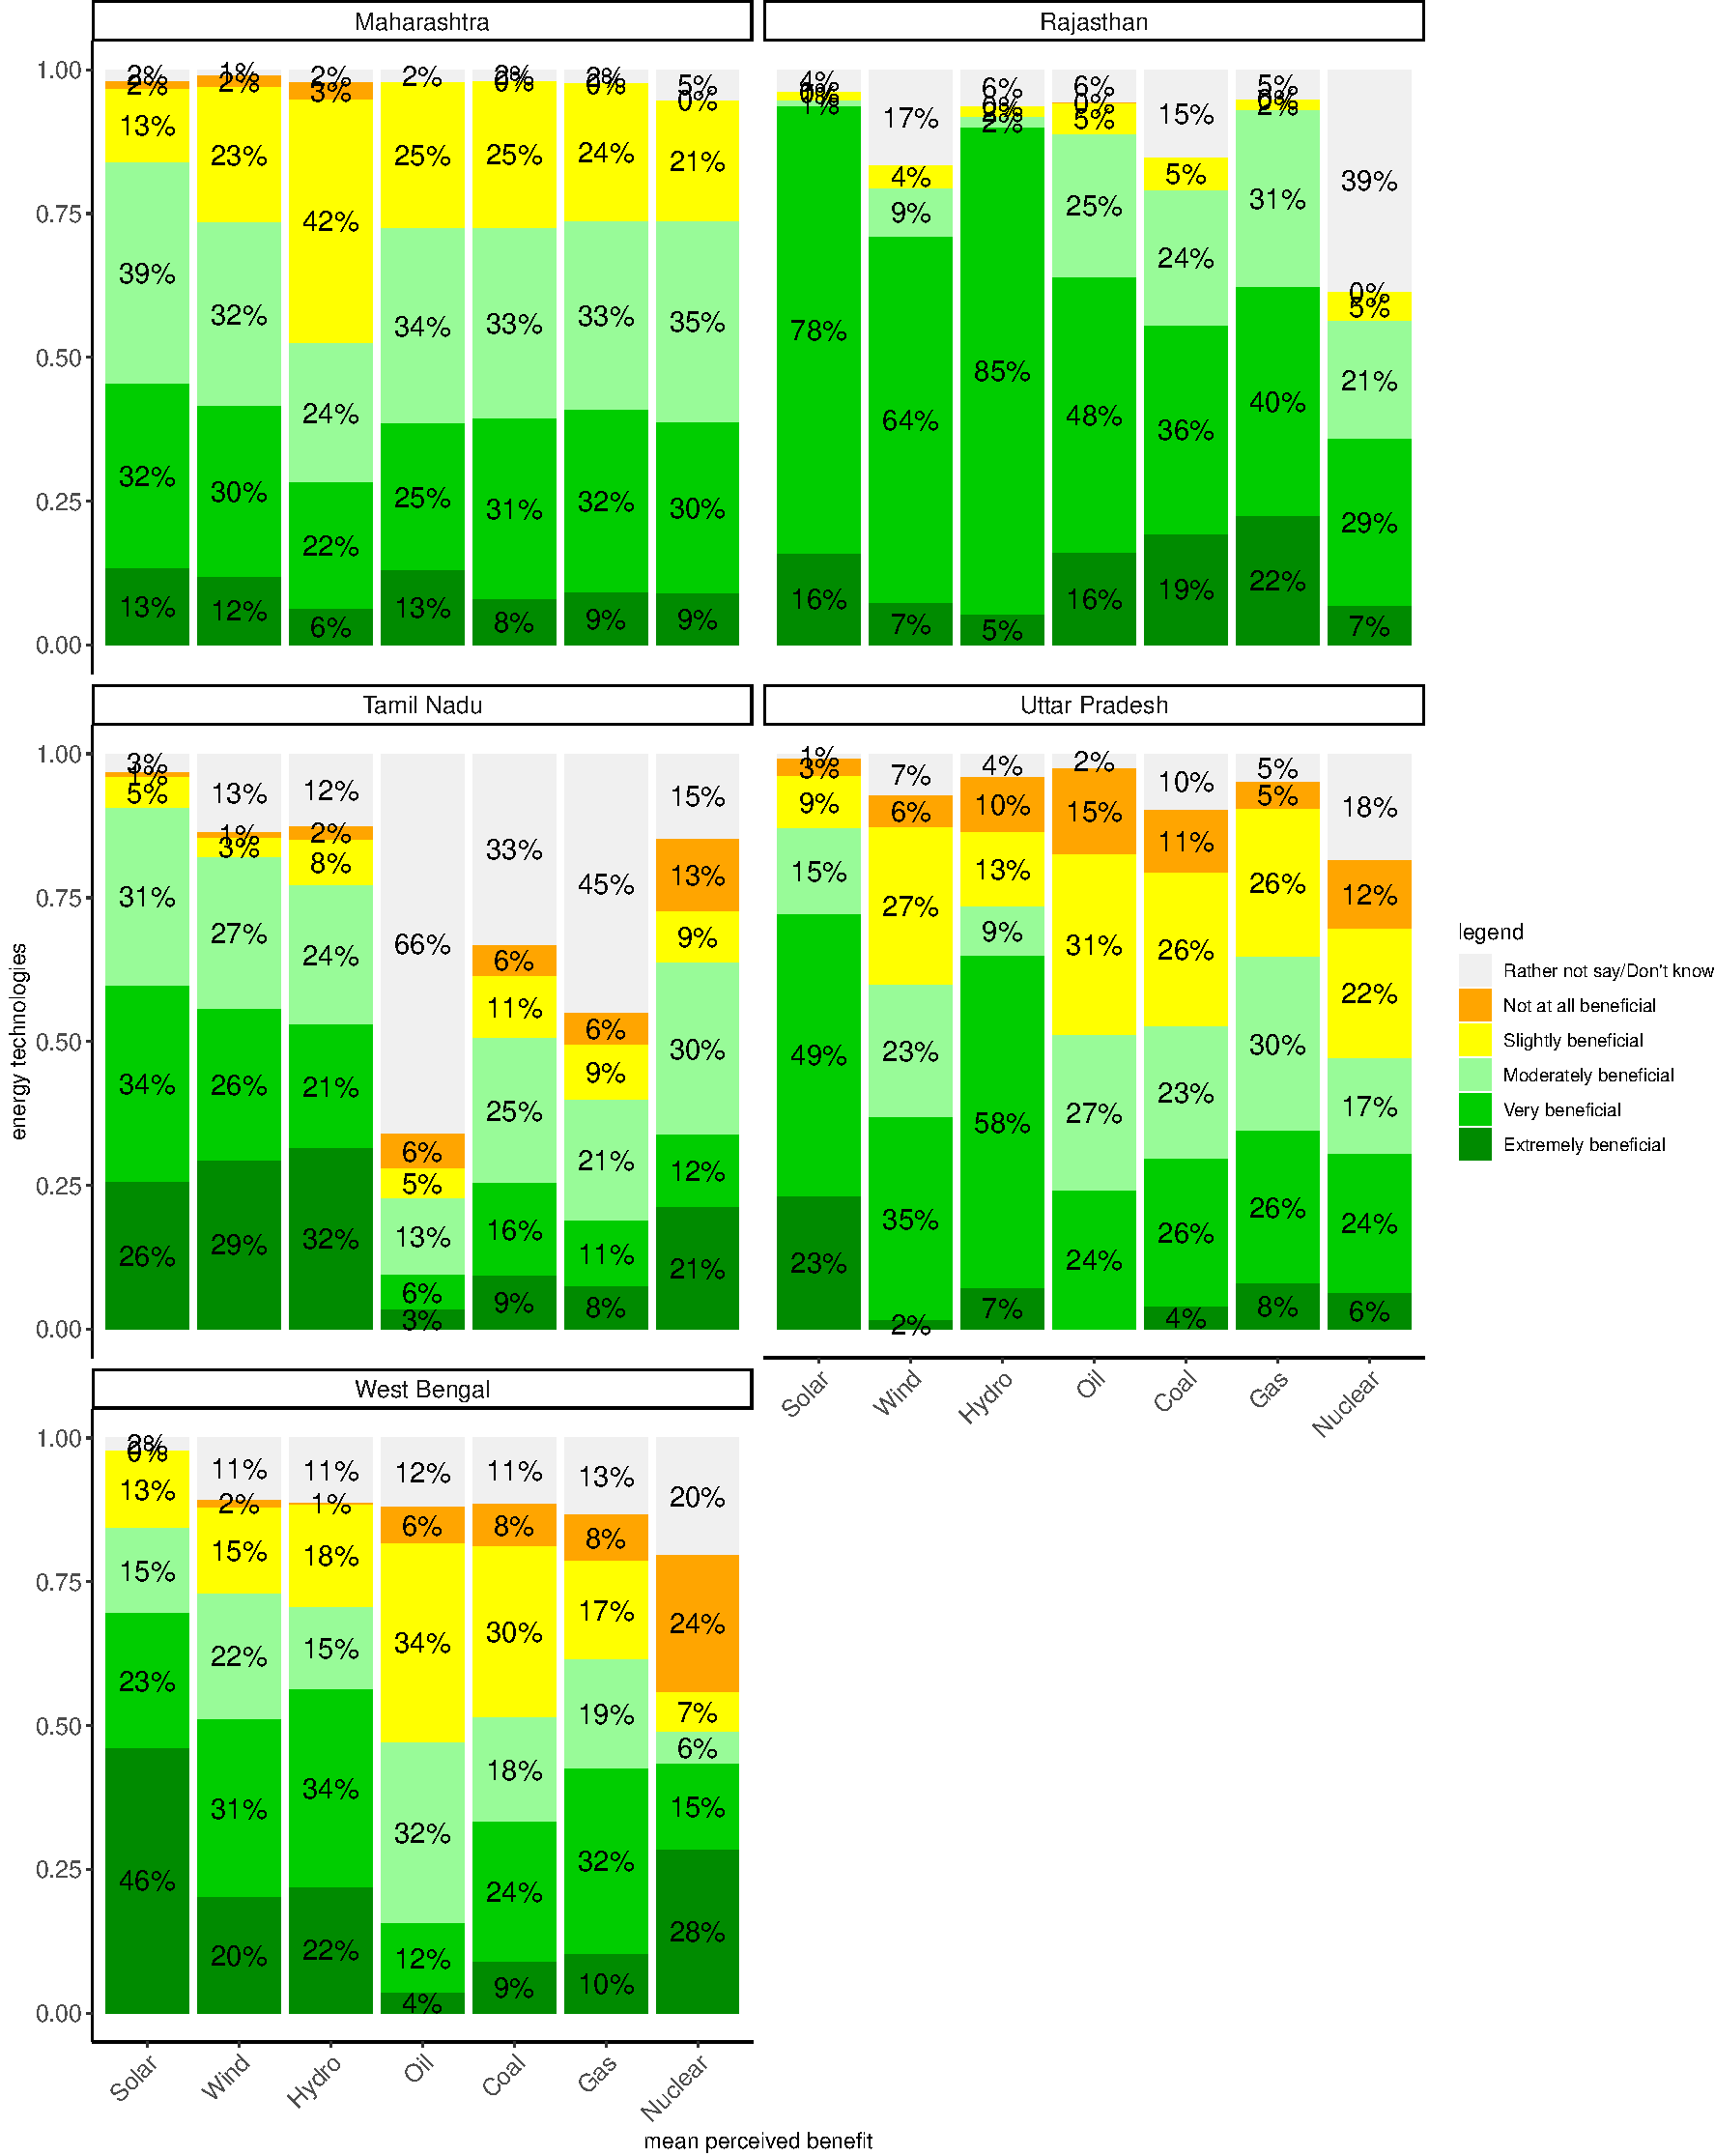
\includegraphics[width=1\linewidth,height=1\textheight]{Significant_results_files/figure-latex/unnamed-chunk-9-1}

\newpage

\hypertarget{how-are-the-perceptions-of-the-risk-of-producing-energy-from-nuclear-fission-different-from-that-of-other-conventional-sources-of-energy-like-coal-or-hydro-power-in-india}{%
\section{How are the perceptions of the risk of producing energy from
nuclear fission different from that of other conventional sources of
energy like coal or hydro power in
India?}\label{how-are-the-perceptions-of-the-risk-of-producing-energy-from-nuclear-fission-different-from-that-of-other-conventional-sources-of-energy-like-coal-or-hydro-power-in-india}}

H : Nuclear energy will be perceived as riskier than other sources of
energy (coal or hydro) in India like in the west.

The box plot shows the differences in Median for perceived risk from all
energy technologies. Nuclear energy has the highest median. The pairwise
wilcox test confirms that these differences are statistically
significant.

The red pairs indicate that there is a statistically significant
difference between the medians of the two groups. White and grey
indicate - no differences between the medians of the two groups.

{[}Wilcox test : the null hypothesis is that there is no significant
difference in the medians of the two groups being compared. The p-value
obtained from the test indicates the probability of observing the
obtained difference in medians (or a more extreme difference) between
the two groups due to chance, if the null hypothesis were true. If the
p-value is below the pre-specified significance level (typically 0.05),
we reject the null hypothesis and conclude that there is a statistically
significant difference between the medians of the two groups. On the
other hand, if the p-value is above the significance level, we fail to
reject the null hypothesis and conclude that there is insufficient
evidence to conclude that there is a significant difference in medians
between the two groups.{]}

\begin{verbatim}
## 
##  Pairwise comparisons using Wilcoxon rank sum test with continuity correction 
## 
## data:  perceivedriskc$perceived_risk and perceivedriskc$technology 
## 
##         Coal    Gas     Hydro   Nuclear Oil     Solar  
## Gas     0.00047 -       -       -       -       -      
## Hydro   < 2e-16 < 2e-16 -       -       -       -      
## Nuclear 2.4e-16 4.9e-07 < 2e-16 -       -       -      
## Oil     6.4e-10 < 2e-16 < 2e-16 < 2e-16 -       -      
## Solar   < 2e-16 < 2e-16 < 2e-16 < 2e-16 < 2e-16 -      
## Wind    < 2e-16 < 2e-16 0.00179 < 2e-16 < 2e-16 < 2e-16
## 
## P value adjustment method: BH
\end{verbatim}

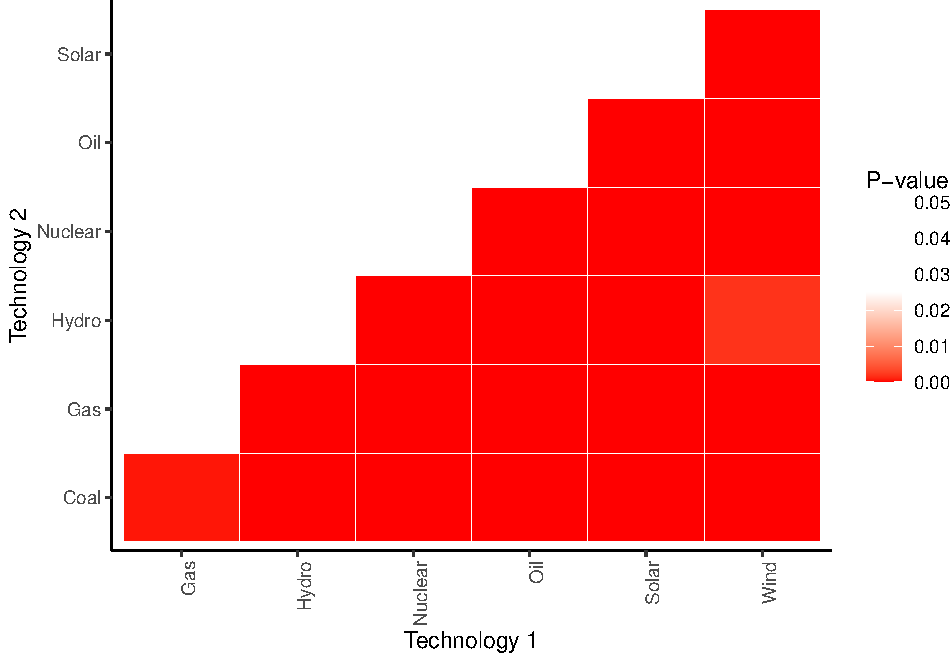
\includegraphics{Significant_results_files/figure-latex/unnamed-chunk-10-1.pdf}
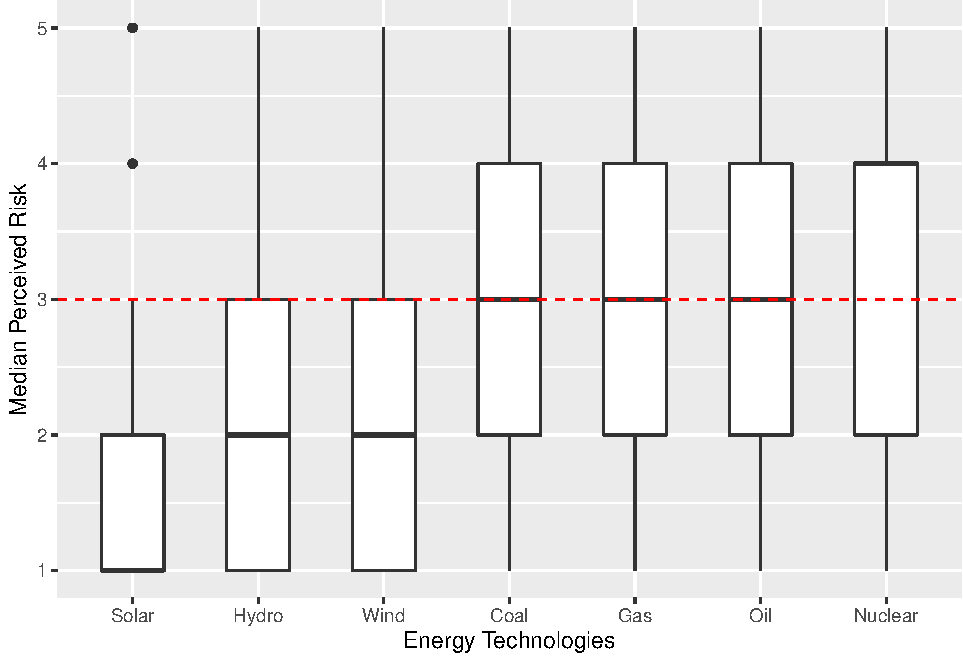
\includegraphics{Significant_results_files/figure-latex/unnamed-chunk-10-2.pdf}

\newpage

\hypertarget{how-do-perceptions-of-benefit-from-nuclear-energy-compare-with-other-source-of-energy}{%
\section{How do perceptions of benefit from nuclear energy compare with
other source of
energy?}\label{how-do-perceptions-of-benefit-from-nuclear-energy-compare-with-other-source-of-energy}}

H : Benefits from all energy technologies will be similar

The box plot shows the differences in Median for perceived benefit from
all energy technologies. The pairwise wilcox test shows if these
differences are statistically significant or not.

The green pairs indicate that there is a statistically significant
difference between the medians of the two groups. White and grey
indicate - no differences between the medians of the two groups.

\begin{verbatim}
## 
##  Pairwise comparisons using Wilcoxon rank sum test with continuity correction 
## 
## data:  perceivedbenefitc$perceived_benefit and perceivedbenefitc$technology 
## 
##         Coal    Gas     Hydro   Nuclear Oil     Solar  
## Gas     0.00338 -       -       -       -       -      
## Hydro   4.2e-10 0.00053 -       -       -       -      
## Nuclear 0.72011 0.02283 8.3e-08 -       -       -      
## Oil     0.07916 1.7e-06 3.7e-16 0.04916 -       -      
## Solar   < 2e-16 < 2e-16 < 2e-16 < 2e-16 < 2e-16 -      
## Wind    3.7e-14 2.3e-06 0.28176 7.1e-11 < 2e-16 2.5e-16
## 
## P value adjustment method: BH
\end{verbatim}

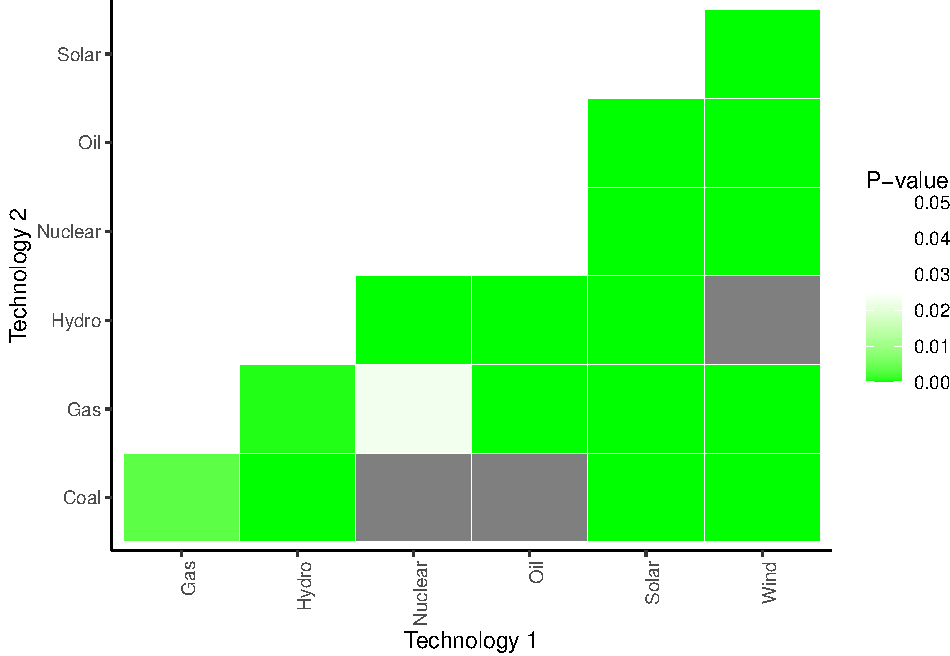
\includegraphics{Significant_results_files/figure-latex/unnamed-chunk-11-1.pdf}
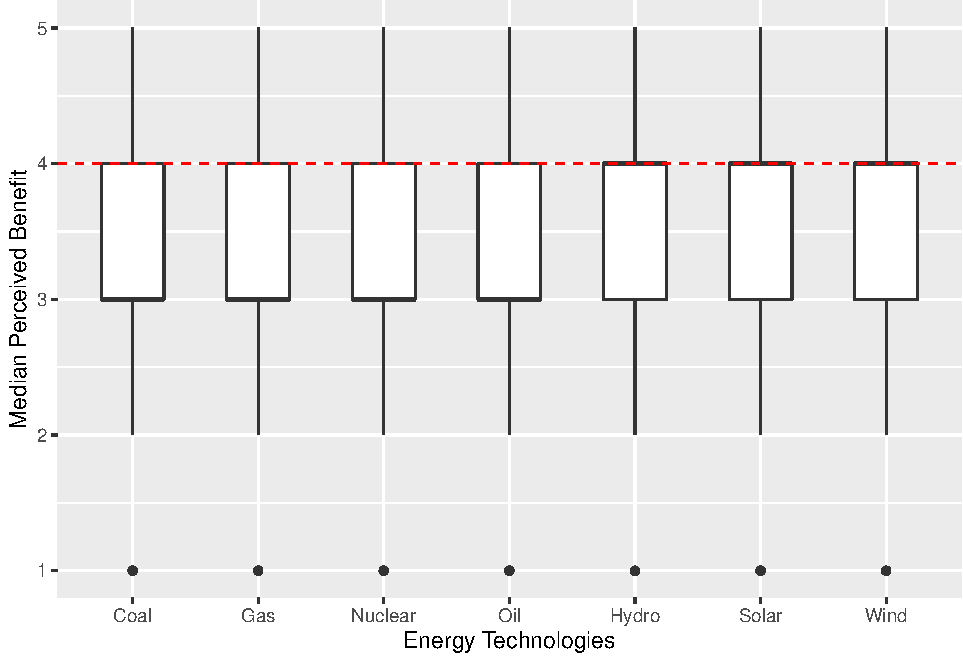
\includegraphics{Significant_results_files/figure-latex/unnamed-chunk-11-2.pdf}

\newpage

\hypertarget{how-do-perception-of-risk-and-perception-of-benefit-compare-with-each-other}{%
\section{How do perception of risk and perception of benefit compare
with each
other?}\label{how-do-perception-of-risk-and-perception-of-benefit-compare-with-each-other}}

Mean Values and Median Values are presented in the graphs below

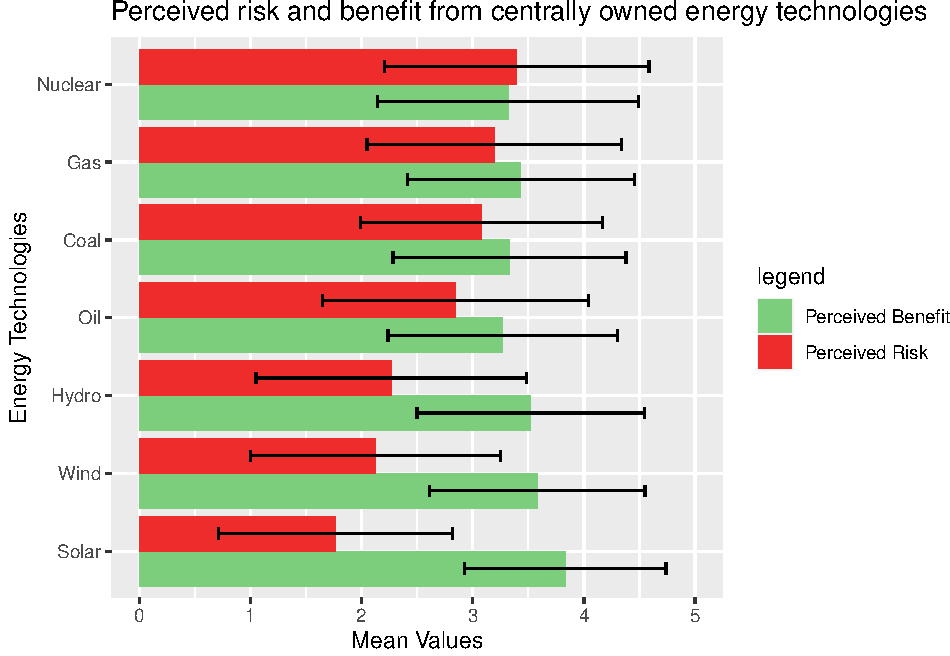
\includegraphics{Significant_results_files/figure-latex/unnamed-chunk-12-1.pdf}

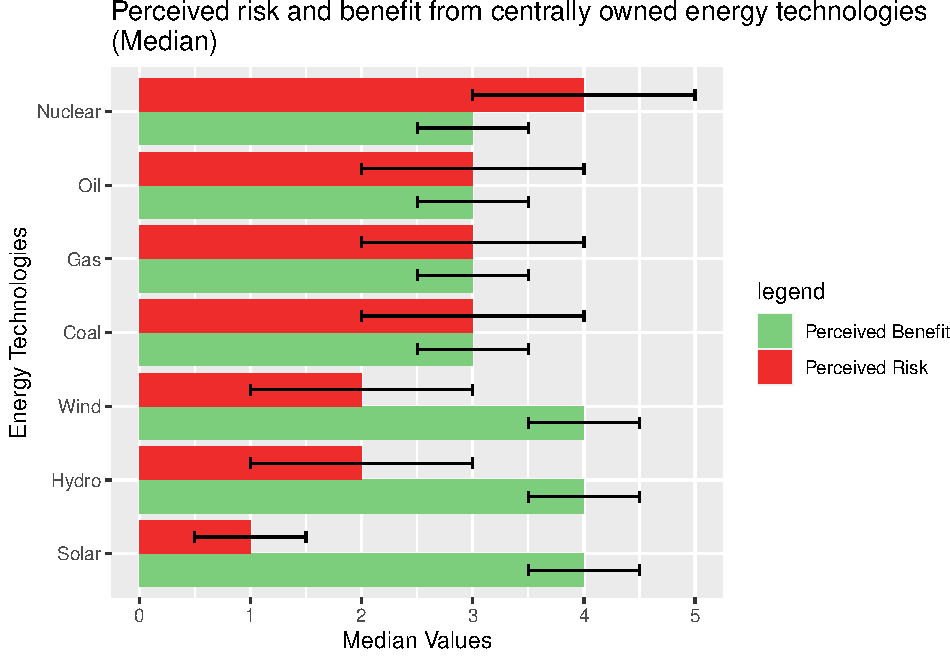
\includegraphics{Significant_results_files/figure-latex/unnamed-chunk-13-1.pdf}

\hypertarget{results-from-wilcoxon-signed-rank-test-used-to-compare-the-median-perceived-risk-and-median-perceived-benefit-from-each-technology.}{%
\subsection{Results from Wilcoxon Signed Rank Test used to compare the
median perceived risk and median perceived benefit from each
technology.}\label{results-from-wilcoxon-signed-rank-test-used-to-compare-the-median-perceived-risk-and-median-perceived-benefit-from-each-technology.}}

Null hypothesis (H0): The median difference between perceived risk and
perceived benefit from each technology is zero.

All p values are less than 0.05 suggesting that the differences observed
above in the graph are statistically significant.

\begin{verbatim}
## $Coal
## [1] 7.780432e-11
## 
## $Gas
## [1] 1.276737e-13
## 
## $Hydro
## [1] 1.157982e-157
## 
## $Nuclear
## [1] 0.002649393
## 
## $Oil
## [1] 8.083808e-33
## 
## $Solar
## [1] 5.50654e-270
## 
## $Wind
## [1] 3.671042e-166
\end{verbatim}

\newpage

\hypertarget{factor-analysis-kahan-scale}{%
\section{Factor Analysis: Kahan
Scale}\label{factor-analysis-kahan-scale}}

Factor Levels for demographic variables - State, age, gender,
urban\_rural, caste and religion First level in each of the variables is
the reference for linear regression models.

\begin{verbatim}
## [1] "Maharashtra"   "Rajasthan"     "Tamil Nadu"    "Uttar Pradesh"
## [5] "West Bengal"
\end{verbatim}

\begin{verbatim}
## [1] "18-24 years old"   "25-34 years old"   "35-44 years old"  
## [4] "45-54 years old"   "55-64 years old"   "65-74 years old"  
## [7] "75 years or older"
\end{verbatim}

\begin{verbatim}
## [1] "Female" "Male"
\end{verbatim}

\begin{verbatim}
## [1] "Rural" "Urban"
\end{verbatim}

\begin{verbatim}
## [1] "Rural" "Urban"
\end{verbatim}

\begin{verbatim}
## [1] "Brahmin" "General" "OBC"     "SC"      "ST"
\end{verbatim}

\begin{verbatim}
## [1] "Agnostism/ Atheism"     "Buddhism"               "Christanity"           
## [4] "Hinduism"               "Islam"                  "Jainism"               
## [7] "Other (Please mention)" "Sikhism"
\end{verbatim}

Before fitting a linear regression model, I conducted factor analysis on
the Kahan scale and the newly developed economic-political value scale.
The results from the Factor Analysis are below.

The Individualism items (indicated by K\_I) were bringing down the
cronbach's alpha values in the Kahan scale. The Alpha for INdividualism-
Communitarian scale was 0.49. After removing the Individualism items
(K\_I) the alpha for this factor was 0.71. The reasons for this could be
that the individualism items are not well adapted to the Indian
population.

I conducted confirmatory factor analysis (CFA) for the Kahan scale (see
Appendix 1) since this a well used scale with theoretical basis for
factor distinctions and also previous studies have used this scale.

\begin{verbatim}
## lavaan 0.6.15 ended normally after 15 iterations
## 
##   Estimator                                         ML
##   Optimization method                           NLMINB
##   Number of model parameters                        15
## 
##   Number of observations                           375
## 
## Model Test User Model:
##                                                       
##   Test statistic                                54.472
##   Degrees of freedom                                13
##   P-value (Chi-square)                           0.000
## 
## Model Test Baseline Model:
## 
##   Test statistic                               676.704
##   Degrees of freedom                                21
##   P-value                                        0.000
## 
## User Model versus Baseline Model:
## 
##   Comparative Fit Index (CFI)                    0.937
##   Tucker-Lewis Index (TLI)                       0.898
## 
## Loglikelihood and Information Criteria:
## 
##   Loglikelihood user model (H0)              -3707.085
##   Loglikelihood unrestricted model (H1)      -3679.849
##                                                       
##   Akaike (AIC)                                7444.170
##   Bayesian (BIC)                              7503.074
##   Sample-size adjusted Bayesian (SABIC)       7455.483
## 
## Root Mean Square Error of Approximation:
## 
##   RMSEA                                          0.092
##   90 Percent confidence interval - lower         0.068
##   90 Percent confidence interval - upper         0.118
##   P-value H_0: RMSEA <= 0.050                    0.003
##   P-value H_0: RMSEA >= 0.080                    0.806
## 
## Standardized Root Mean Square Residual:
## 
##   SRMR                                           0.046
## 
## Parameter Estimates:
## 
##   Standard errors                             Standard
##   Information                                 Expected
##   Information saturated (h1) model          Structured
## 
## Latent Variables:
##                    Estimate  Std.Err  z-value  P(>|z|)   Std.lv  Std.all
##   KahanS =~                                                             
##     K_SHARM           0.690    0.062   11.043    0.000    0.690    0.628
##     K_SLIMCHOI        0.738    0.064   11.570    0.000    0.738    0.659
##     K_SPROTECT        0.495    0.064    7.770    0.000    0.495    0.453
##   KahanH =~                                                             
##     K_HEQUAL          0.743    0.061   12.197    0.000    0.743    0.628
##     K_ERADEQ1        -0.796    0.052  -15.207    0.000   -0.796   -0.750
##     K_EWEALTH        -0.663    0.060  -11.095    0.000   -0.663   -0.580
##     K_ERADEQ2        -0.840    0.056  -14.990    0.000   -0.840   -0.741
## 
## Covariances:
##                    Estimate  Std.Err  z-value  P(>|z|)   Std.lv  Std.all
##   KahanS ~~                                                             
##     KahanH           -0.772    0.049  -15.878    0.000   -0.772   -0.772
## 
## Variances:
##                    Estimate  Std.Err  z-value  P(>|z|)   Std.lv  Std.all
##    .K_SHARM           0.730    0.073    9.973    0.000    0.730    0.605
##    .K_SLIMCHOI        0.709    0.077    9.272    0.000    0.709    0.565
##    .K_SPROTECT        0.952    0.078   12.281    0.000    0.952    0.795
##    .K_HEQUAL          0.850    0.074   11.544    0.000    0.850    0.606
##    .K_ERADEQ1         0.493    0.053    9.367    0.000    0.493    0.438
##    .K_EWEALTH         0.865    0.072   12.026    0.000    0.865    0.663
##    .K_ERADEQ2         0.578    0.060    9.581    0.000    0.578    0.450
##     KahanS            1.000                               1.000    1.000
##     KahanH            1.000                               1.000    1.000
\end{verbatim}

RMSEA - between 0.05 and 0.08 (reasonable fit), less than 0.05 close fit
and greater than 0.10 is poor fit CFI - greater than 0.90 or 0.95
indicates good fit TFI - CFI\textgreater TFI \textgreater0.90 -
indicates good fit

After having removed a few variables that had very low loading, the
model is now a good fit. Some of the Individualistic variables just
don't fit. Final scale variables:

KahanS(Individualism - Communitarian) = K\_SHARM + K\_SLIMCHOI +
K\_SPROTECT KahanH(Hierarchy- Egalitarian) =K\_HEQUAL+ K\_ERADEQ1 +
K\_EWEALTH + K\_ERADEQ2

The Cronabch alpha for this final scale was 0.75.

\newpage

\hypertarget{factor-analysis-new-eco-political-scale}{%
\section{Factor Analysis: New Eco-political
Scale}\label{factor-analysis-new-eco-political-scale}}

Then I conducted Factor Analysis on all eco-political values(see
Appendix 2). The Cronbach's alpha for the scale was high at 0.785
(almost 0.8).

The scale reduced to two factors which I named as 1) People Centered
Development and 2) Nationalist Development. The final scale with two
factors include the following

\textbf{MR1 People Centered Development: Pdevelop}

HEALTHNUCLEAR - Nuclear energy poses a great risk to the health of
people living around it.

BEAUTYNUCLEAR - Nuclear energy spoils the natural beauty of the
landscape.

MECHANISATION - Rapid mechanization of work is taking away jobs from
workers in this country.

INDUSTRYSMALL - Large corporations are destroying the local industries
in India and benefiting only a handful of people.

DISPLACENUCLEAR- Nuclear energy is leading to displacement of people
from their land.

POLLUTENUCLEAR- Nuclear energy increases pollution of air/water/land.

OWNERREG- Regardless of ownership, the government should pass strong
regulations and implement them.

\textbf{MR2 Nationalist Development: Ndevelop}

DEVNUCLEAR - Nuclear energy pushes forward the country's development.

PRIDENUCLEAR- I would be proud if my community used nuclear energy.

NPRIDENUCLEAR- Nuclear energy is a mark of pride for our nation.

PROSPERNUCLEAR-Nuclear energy brings economic prosperity to the
surrounding regions.

INDUSTRYLARGE- Large scale industries are required for the development
of the country that will benefit everyone.

The results of the factor analysis are below:

\begin{verbatim}
## 
## Reliability analysis   
##  raw_alpha std.alpha G6(smc) average_r S/N   ase mean   sd median_r
##        0.8       0.8    0.84      0.14   4 0.015  3.3 0.47     0.15
\end{verbatim}

\begin{verbatim}
## Factor Analysis using method =  minres
## Call: fa(r = ecopolall, nfactors = 2, rotate = "varimax")
## Standardized loadings (pattern matrix) based upon correlation matrix
##                 item   MR1   MR2     h2   u2 com
## HEALTHNUCLEAR     17  0.61       0.3880 0.61 1.1
## BEAUTYNUCLEAR     19  0.60       0.3679 0.63 1.1
## MECHANISATION      2  0.57       0.3892 0.61 1.4
## INDUSTRYSMALL      6 -0.56       0.3280 0.67 1.1
## DISPLACENUCLEAR   15  0.54       0.3555 0.64 1.4
## POLLUTENUCLEAR    16  0.53       0.2811 0.72 1.0
## OWNERREG          14 -0.50       0.2848 0.72 1.3
## ENVOVERDEV         9             0.1403 0.86 1.1
## DECISIONDECEN      3             0.1058 0.89 1.0
## OWNERPUB          13             0.1178 0.88 1.7
## DECISIONCEN        4             0.1160 0.88 1.8
## OWNERPVT          11             0.0610 0.94 1.0
## ECONOMYLOCAL       8             0.0243 0.98 1.1
## DEVOVERENV        10             0.0015 1.00 1.2
## DEVNUCLEAR        22        0.65 0.4530 0.55 1.1
## PRIDENUCLEAR      20        0.61 0.4108 0.59 1.2
## NPRIDENUCLEAR     21        0.57 0.3608 0.64 1.2
## PROSPERNUCLEAR    23        0.55 0.3267 0.67 1.1
## INDUSTRYLARGE      5        0.43 0.2386 0.76 1.5
## RELYNUCLEAR       24             0.1590 0.84 1.1
## WEALTHLIM          1             0.2036 0.80 1.7
## ECONOMYGLOBAL      7             0.2480 0.75 2.0
## JOBSNUCLEAR       18             0.1933 0.81 1.9
## OWNERNOREG        12             0.0565 0.94 1.9
## 
##                        MR1  MR2
## SS loadings           3.13 2.49
## Proportion Var        0.13 0.10
## Cumulative Var        0.13 0.23
## Proportion Explained  0.56 0.44
## Cumulative Proportion 0.56 1.00
## 
## Mean item complexity =  1.3
## Test of the hypothesis that 2 factors are sufficient.
## 
## The degrees of freedom for the null model are  276  and the objective function was  6.02 with Chi Square of  2198.62
## The degrees of freedom for the model are 229  and the objective function was  2.43 
## 
## The root mean square of the residuals (RMSR) is  0.08 
## The df corrected root mean square of the residuals is  0.09 
## 
## The harmonic number of observations is  375 with the empirical chi square  1292.99  with prob <  8.6e-148 
## The total number of observations was  375  with Likelihood Chi Square =  884.44  with prob <  9.5e-78 
## 
## Tucker Lewis Index of factoring reliability =  0.587
## RMSEA index =  0.087  and the 90 % confidence intervals are  0.081 0.094
## BIC =  -472.83
## Fit based upon off diagonal values = 0.83
## Measures of factor score adequacy             
##                                                    MR1  MR2
## Correlation of (regression) scores with factors   0.89 0.88
## Multiple R square of scores with factors          0.80 0.77
## Minimum correlation of possible factor scores     0.60 0.53
\end{verbatim}

\newpage

\hypertarget{linear-regression-4-models.}{%
\section{Linear Regression: 4
Models.}\label{linear-regression-4-models.}}

Then I ran 4 linear regression models adding more variables every time.
The results of the linear regression models are below.

\begingroup\setlength{\tabcolsep}{1pt}\renewcommand{\arraystretch}{0.7}

\% Table created by stargazer v.5.2.3 by Marek Hlavac, Social Policy
Institute. E-mail: marek.hlavac at gmail.com \% Date and time: Mon, Jul
17, 2023 - 13:22:23

\begin{table}[!htbp] \centering 
  \caption{Results from 4 linear regression models} 
  \label{} 
\begin{tabular}{@{\extracolsep{5pt}}lcccc} 
\\[-1.8ex]\hline 
\hline \\[-1.8ex] 
 & \multicolumn{4}{c}{\textit{Dependent variable:}} \\ 
\cline{2-5} 
\\[-1.8ex] & \multicolumn{4}{c}{Risky\_Nuclear} \\ 
\\[-1.8ex] & (1) & (2) & (3) & (4)\\ 
\hline \\[-1.8ex] 
 Uppercaste & $-$0.109 & $-$0.032 & $-$0.016 & $-$0.038 \\ 
  & (0.119) & (0.111) & (0.108) & (0.108) \\ 
  & & & & \\ 
 Male & 0.226$^{**}$ & $-$0.105 & $-$0.095 & $-$0.072 \\ 
  & (0.115) & (0.123) & (0.120) & (0.119) \\ 
  & & & & \\ 
 Hindu & 0.054 & $-$0.033 & $-$0.038 & $-$0.003 \\ 
  & (0.130) & (0.122) & (0.118) & (0.118) \\ 
  & & & & \\ 
 UrbanUrban & $-$0.242$^{**}$ & 0.022 & $-$0.018 & $-$0.002 \\ 
  & (0.111) & (0.119) & (0.116) & (0.116) \\ 
  & & & & \\ 
 age25-34 years old &  & $-$0.094 & $-$0.079 & $-$0.046 \\ 
  &  & (0.124) & (0.121) & (0.120) \\ 
  & & & & \\ 
 age35-44 years old &  & $-$0.066 & $-$0.103 & $-$0.118 \\ 
  &  & (0.151) & (0.148) & (0.147) \\ 
  & & & & \\ 
 age45-54 years old &  & 0.083 & 0.121 & 0.158 \\ 
  &  & (0.256) & (0.250) & (0.248) \\ 
  & & & & \\ 
 age55-64 years old &  & 0.109 & 0.240 & 0.369 \\ 
  &  & (0.495) & (0.483) & (0.479) \\ 
  & & & & \\ 
 age65-74 years old &  & 1.183$^{**}$ & 1.260$^{**}$ & 1.167$^{**}$ \\ 
  &  & (0.564) & (0.549) & (0.545) \\ 
  & & & & \\ 
 age75 years or older &  & 0.076 & $-$0.194 & $-$0.363 \\ 
  &  & (0.960) & (0.936) & (0.929) \\ 
  & & & & \\ 
 StateRajasthan &  & 0.659$^{***}$ & 0.382$^{**}$ & 0.136 \\ 
  &  & (0.163) & (0.171) & (0.186) \\ 
  & & & & \\ 
 StateTamil Nadu &  & 1.372$^{***}$ & 1.030$^{***}$ & 0.941$^{***}$ \\ 
  &  & (0.238) & (0.243) & (0.283) \\ 
  & & & & \\ 
 StateUttar Pradesh &  & 0.364$^{*}$ & 0.060 & $-$0.036 \\ 
  &  & (0.195) & (0.201) & (0.202) \\ 
  & & & & \\ 
 StateWest Bengal &  & 1.474$^{***}$ & 0.981$^{***}$ & 0.774$^{***}$ \\ 
  &  & (0.215) & (0.234) & (0.247) \\ 
  & & & & \\ 
 KahanS &  &  & $-$0.272$^{**}$ & $-$0.213 \\ 
  &  &  & (0.134) & (0.135) \\ 
  & & & & \\ 
 KahanH &  &  & 0.053 & $-$0.049 \\ 
  &  &  & (0.125) & (0.127) \\ 
  & & & & \\ 
 Pdevelop &  &  &  & 0.187$^{**}$ \\ 
  &  &  &  & (0.078) \\ 
  & & & & \\ 
 Ndevelop &  &  &  & 0.178$^{***}$ \\ 
  &  &  &  & (0.064) \\ 
  & & & & \\ 
 Constant & 3.184$^{***}$ & 3.029$^{***}$ & 3.172$^{***}$ & 3.192$^{***}$ \\ 
  & (0.161) & (0.162) & (0.160) & (0.161) \\ 
  & & & & \\ 
\hline \\[-1.8ex] 
Observations & 375 & 375 & 375 & 375 \\ 
R$^{2}$ & 0.033 & 0.216 & 0.262 & 0.282 \\ 
Adjusted R$^{2}$ & 0.023 & 0.185 & 0.229 & 0.246 \\ 
Residual Std. Error & 1.033 (df = 370) & 0.944 (df = 360) & 0.918 (df = 358) & 0.908 (df = 356) \\ 
F Statistic & 3.187$^{**}$ (df = 4; 370) & 7.078$^{***}$ (df = 14; 360) & 7.926$^{***}$ (df = 16; 358) & 7.787$^{***}$ (df = 18; 356) \\ 
\hline 
\hline \\[-1.8ex] 
\textit{Note:}  & \multicolumn{4}{r}{$^{*}$p$<$0.1; $^{**}$p$<$0.05; $^{***}$p$<$0.01} \\ 
\end{tabular} 
\end{table} 
\endgroup

Key observations:

\textbf{1. Demographic effects:} The impact of demographic
characteristics on the perceived risk from Nuclear Energy appears to be
small. The adjusted R-squared of the first model, which includes only
demographic variables, is 0.023, indicating that these variables explain
just over 2\% of the variance in perceived risk.

\textbf{2. Age effects:} In Model 2, where age groups are added, there
is a distinct change in the perceived risk from nuclear energy as age
increases. Interestingly, only the age group 65-74 shows a significant
increase in perceived risk, compared to the reference age group (18-25
years).

\textbf{3. Gender effects:} In the initial model, being male is
positively associated with higher perceived risk from nuclear energy.
However, the significance of this association diminishes when age and
state variables are included in the model, suggesting that the
relationship between gender and perceived risk may be influenced by
these factors.

\textbf{4. State effects:} Both exploratory visualizations and
regression models strongly suggest that the respondents' state of
residence significantly influences their perceived risk from nuclear
energy. The comparison state is Maharashtra. The coefficients for the
other states can be interpreted as the difference in perceived risk from
each state compared to Maharashtra, holding all else constant.

\textbf{5. Kahan scale effects:} Among the Kahan scale variables, only
the individualism factor is statistically significant in the third
model. This suggests that individuals scoring high on the individualism
scale perceive nuclear energy as less risky.

\textbf{6. Eco-political scale effects:} When we introduce the
eco-political scale, the effect of the individualism factor from the
Kahan scale loses its significance. This could suggest that the
eco-political scale is capturing some aspect of the risk perception
related to individualism. The two factors of the eco-political scale
both have a statistically significant impact on the perceived risk,
indicating that these eco-political beliefs play an important role in
shaping risk perceptions.

\newpage

\hypertarget{system-of-government-items}{%
\section{System of Government Items}\label{system-of-government-items}}

The governance items were not going very well with the items in the
eco-political value scale. So I kept them separate. Below are some
exploratory graphs on them. In these graphs high values contain somewhat
agree(4) or strongly agree(5) and low contains strongly disagree(1),
somewhat disagree(2).

\hypertarget{perceived-risk-by-support-for-democratic-government}{%
\subsection{Perceived risk by Support for Democratic
government}\label{perceived-risk-by-support-for-democratic-government}}

\begin{verbatim}
##    grouped_demo technology     mean   n        sd
## 1          high       Coal 3.177236 721 1.1340749
## 2          high        Gas 3.246732 721 1.2161915
## 3          high      Hydro 2.175079 721 1.2603858
## 4          high    Nuclear 3.372093 721 1.2560982
## 5          high        Oil 2.840070 721 1.3178397
## 6          high      Solar 1.588410 721 1.0140307
## 7          high       Wind 2.032432 721 1.2072407
## 8           low       Coal 2.961290 157 1.0057230
## 9           low        Gas 3.026144 157 1.0447092
## 10          low      Hydro 2.279221 157 1.0064936
## 11          low    Nuclear 3.075862 157 1.0806554
## 12          low        Oil 3.026144 157 0.9996559
## 13          low      Solar 2.283871 157 1.0675548
## 14          low       Wind 2.337748 157 0.9858155
\end{verbatim}

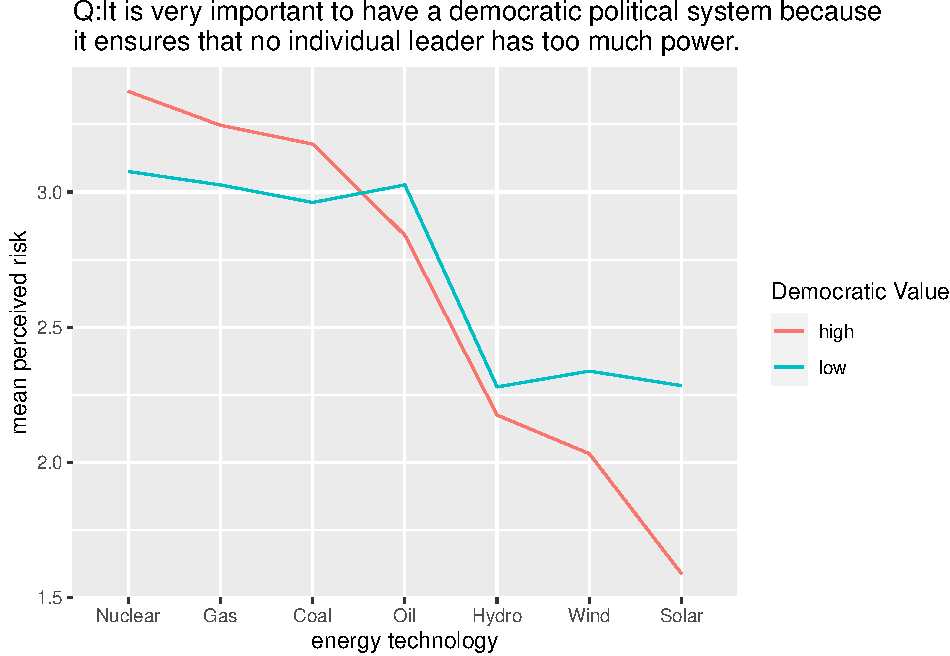
\includegraphics{Significant_results_files/figure-latex/unnamed-chunk-19-1.pdf}

\newpage

\hypertarget{perceived-risk-by-support-for-totalitarian-government}{%
\subsection{Perceived risk by Support for Totalitarian
government}\label{perceived-risk-by-support-for-totalitarian-government}}

\begin{verbatim}
##    grouped_total technology     mean   n       sd
## 1           high       Coal 3.086735 466 1.200012
## 2           high        Gas 3.217848 466 1.300727
## 3           high      Hydro 2.209877 466 1.239970
## 4           high    Nuclear 3.403599 466 1.255539
## 5           high        Oil 3.296512 466 1.114123
## 6           high      Solar 1.692841 466 1.023053
## 7           high       Wind 2.084615 466 1.171872
## 8            low       Coal 3.229814 344 1.042693
## 9            low        Gas 3.223975 344 1.080755
## 10           low      Hydro 2.103030 344 1.252956
## 11           low    Nuclear 3.360902 344 1.186963
## 12           low        Oil 2.677524 344 1.307438
## 13           low      Solar 1.783383 344 1.111609
## 14           low       Wind 1.966997 344 1.127134
\end{verbatim}

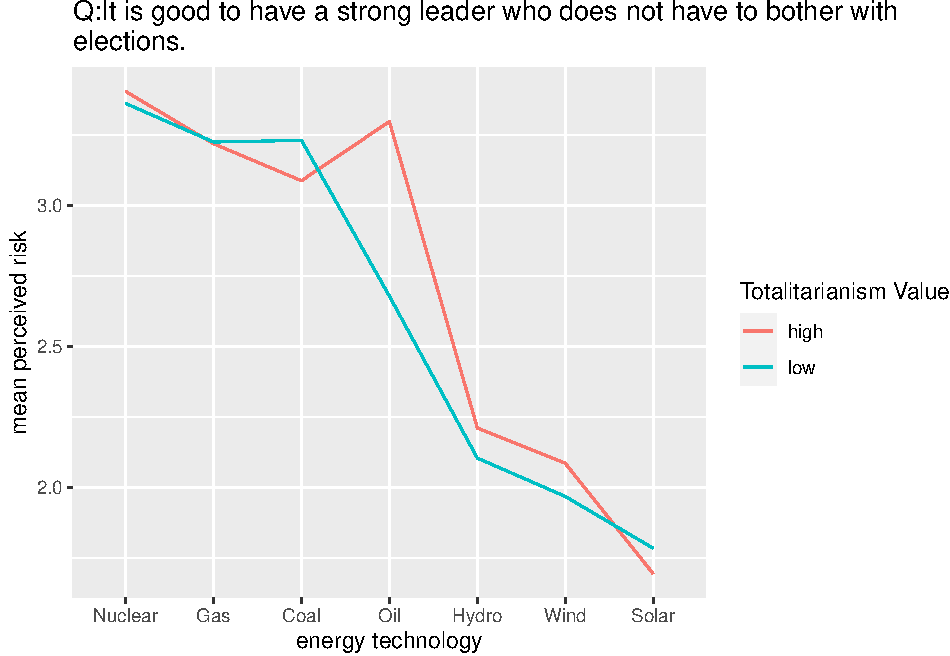
\includegraphics{Significant_results_files/figure-latex/unnamed-chunk-20-1.pdf}

\newpage

\hypertarget{perceived-risk-by-support-for-technocratic-government}{%
\subsection{Perceived risk by Support for Technocratic
government}\label{perceived-risk-by-support-for-technocratic-government}}

\begin{verbatim}
##    grouped_techno technology     mean   n       sd
## 1            high       Coal 3.177215 626 1.110419
## 2            high        Gas 3.280961 626 1.204385
## 3            high      Hydro 2.133449 626 1.232323
## 4            high    Nuclear 3.491803 626 1.240957
## 5            high        Oil 2.889109 626 1.328705
## 6            high      Solar 1.638047 626 1.016873
## 7            high       Wind 2.026616 626 1.180498
## 8             low       Coal 3.107143 190 1.083550
## 9             low        Gas 3.238372 190 1.132267
## 10            low      Hydro 2.394286 190 1.178822
## 11            low    Nuclear 3.151899 190 1.135289
## 12            low        Oil 3.222930 190 1.065777
## 13            low      Solar 1.978261 190 1.106150
## 14            low       Wind 2.248447 190 1.112604
\end{verbatim}

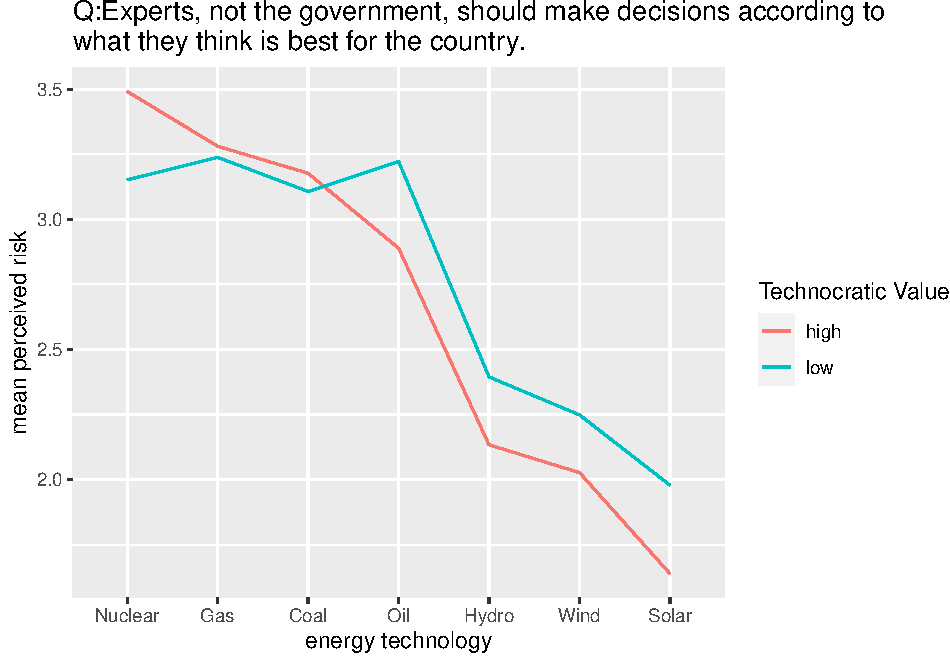
\includegraphics{Significant_results_files/figure-latex/unnamed-chunk-21-1.pdf}

\newpage

\hypertarget{perceived-risk-by-support-for-religious-government}{%
\subsection{Perceived risk by Support for Religious
government}\label{perceived-risk-by-support-for-religious-government}}

\begin{verbatim}
##    grouped_religion technology     mean   n        sd
## 1              high       Coal 3.025189 449 1.1500418
## 2              high        Gas 3.426630 449 1.1364880
## 3              high      Hydro 2.215385 449 1.1493909
## 4              high    Nuclear 3.120805 449 1.3653369
## 5              high        Oil 2.965714 449 1.1795640
## 6              high      Solar 1.702179 449 1.0361992
## 7              high       Wind 2.217105 449 1.2045993
## 8               low       Coal 3.250000 427 1.0474290
## 9               low        Gas 3.072165 427 1.2093300
## 10              low      Hydro 2.045918 427 1.2481941
## 11              low    Nuclear 3.525568 427 1.1039554
## 12              low        Oil 2.759003 427 1.3081298
## 13              low      Solar 1.592233 427 0.9709843
## 14              low       Wind 1.882199 427 1.0888350
\end{verbatim}

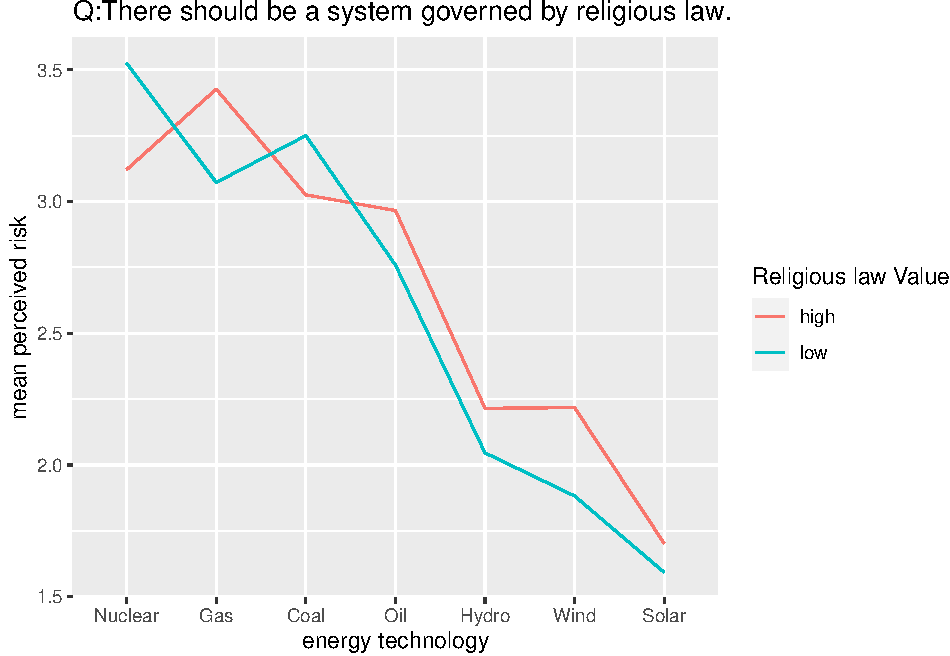
\includegraphics{Significant_results_files/figure-latex/unnamed-chunk-22-1.pdf}

\newpage

\hypertarget{appendix1}{%
\section{Appendix1}\label{appendix1}}

\textbf{Kahan et al (2007) scale}

Individualism - Communitarinism

\begin{itemize}
\tightlist
\item
  \textbf{K\_IINTRFER} The government interferes far too much in our
  everyday lives.
\item
  \textbf{K\_IPRIVACY} The government should stop telling people how to
  live their lives.
\item
  \textbf{K\_IPROTECT} It's not the government's business to try to
  protect people from themselves.
\item
  \textbf{K\_SHARM} Sometimes the government needs to make laws that
  keep people from hurting themselves.
\item
  \textbf{K\_SLIMCHOI} The government should put limits on the choices
  individuals can make so they don't get in the way of what's good for
  society.
\item
  \textbf{K\_SPROTECT} The government should do more to advance
  society's goals, even if that means limiting the freedom and choices
  of individuals.
\end{itemize}

Hierarchy -Egalitarianism

\begin{itemize}
\tightlist
\item
  \textbf{K\_HEQUAL} We have gone too far in pushing equal rights in
  this country.
\item
  \textbf{K\_HREVDIS1} Nowadays it seems like there is just as much
  discrimination against upper castes as there is against Dalits.
\item
  \textbf{K\_EDISCRIM} Discrimination against minorities is still a very
  serious problem in our society.
\item
  \textbf{K\_ERADEQ1} We need to dramatically reduce inequalities
  between the rich and the poor.
\item
  \textbf{K\_EWEALTH} Our society would be better off if the
  distribution of wealth was more equal.
\item
  \textbf{K\_ERADEQ2} We need to dramatically reduce inequalities
  between men and women.
\end{itemize}

\newpage

\hypertarget{appendix2}{%
\section{Appendix2}\label{appendix2}}

\textbf{New Eco-pol values scale}

\begin{itemize}
\item
  \textbf{DISPLACENUCLER} Nuclear energy is leading to displacement of
  people from their land
\item
  \textbf{BEAUTYNUCLEAR} Nuclear energy spoils the natural beauty of the
  landscape
\item
  \textbf{POLLUTENUCLEAR} Nuclear energy increases pollution of
  air/water/land
\item
  \textbf{HEALTHNUCLEAR} Nuclear energy poses a great risk to the health
  of people living around it
\item
  \textbf{JOBSNUCLEAR} Nuclear energy will bring jobs to the local
  community
\item
  \textbf{PRIDENUCLEAR} I would be proud if my community used nuclear
  energy
\item
  \textbf{NPRIDENUCLEAR} Nuclear energy is a mark of pride for our
  nation
\item
  \textbf{DEVNUCLEAR} Nuclear energy pushes forward the country's
  development
\item
  \textbf{PROSPERNUCLEAR} Nuclear energy brings economic prosperity to
  the surrounding regions
\item
  \textbf{RELYNUCLEAR} I don't like the idea that I have to rely on the
  government for electricity from nuclear energy
\item
  \textbf{DECISIONDECEN} Local politicians shouldn't have to ask
  permission from the central government to implement policies
\item
  \textbf{DECISIONCEN} Laws and policies would be implemented more
  smoothly if more power lay with the central government.
\item
  \textbf{INDUSTRYLARGE} Large scale industries are required for the
  development of the country that will benefit everyone
\item
  \textbf{ECONOMYLOCAL} India would be better off if foreign companies
  didn't come to here
\item
  \textbf{DEVOVERENV} Economic growth and creating jobs should be
  prioritized over environmental protection
\item
  \textbf{INDUSTRYSMALL} Large corporations are destroying the local
  industries in India and benefiting only a handful of people.
\item
  \textbf{WEALTHLIM} A limit should be put to how much wealth a person
  can amass
\item
  \textbf{ECONOMYGLOBAL} Foreign companies have led to a range of
  benefits for the Indian people and society
\item
  \textbf{OWNERPVT} All businesses and industries should be owned
  privatel
\item
  \textbf{OWNERPUB} The government should own most large businesses and
  industrie
\item
  \textbf{ENVOVERDEV} Polluting industries that spoil the environment
  should be shut down even if it costs people their jo
\item
  \textbf{OWNERREG} Regardless of ownership, the government should pass
  strong regulations and implement them
\item
  \textbf{MECHANISATION} Rapid mechanization of work is taking away jobs
  from workers in this country
\item
  \textbf{OWNERNOREG} There is too much red-tape and the government
  should not interfere with businesses and industries
\end{itemize}

\end{document}
